\section{Лабораторная работа №3\\
\Large Испытание бруса на изгиб}

Цель работы: экспериментальная проверка теоретического закона распределения напряжений в поперечном сечении бруса при его изгибе с использованием метода тензометрии; измерение величины прогиба.

Оборудование и инструменты: универсальная испытательная машина УММ-5, измеритель статической деформации, комплект проволочных тензодатчиков, универсальный измеритель перемещений часового типа, штангенциркуль, линейка.

\subsection{Теоретические сведения}

\begin{figure}[!ht]
    \centering
    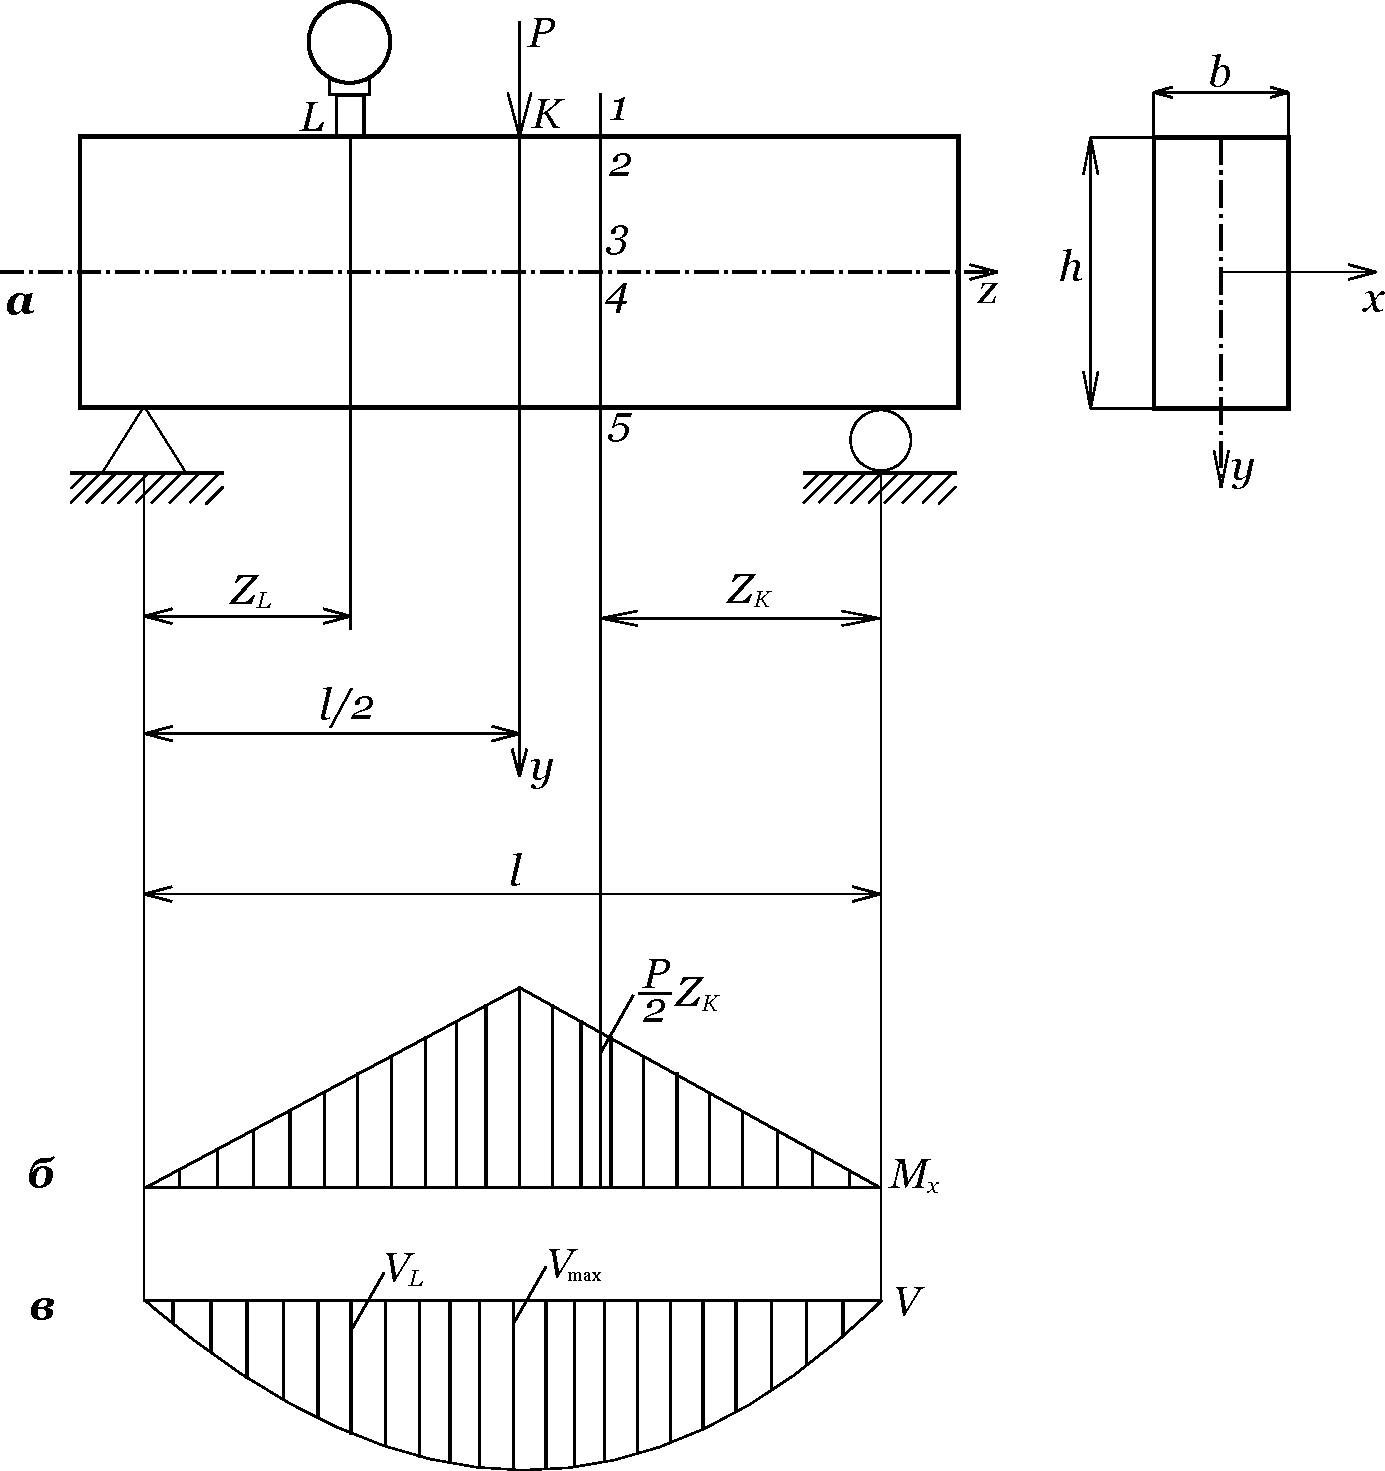
\includegraphics[width=0.8\textwidth]{beam-scheme.pdf}
    \caption{Схема испытания бруса на изгиб:
        а "--- схема нагружения (1\==5 "--- тензодатчики);
        б "--- эпюра изгибающего момента;
        в "--- эпюра прогиба.
    }
    \label{fig:beam-scheme}
\end{figure}

Нормальное напряжение в произвольной точке сечения бруса
\[
    \sigma = \frac{M_x}{I_x}y~[МПа],
\]
где $M_x$ "--- изгибающий момент, $I_x$ "--- осевой момент.

\[
    \sigma_{теор} = \frac{6 P}{b h^3} z y,
\]
где $y$ и $z$ "--- координаты выбранной точки поперечного сечения.

\[
    V_{теор} = \frac{M_x}{E I_x},
\]
где $E$ "--- модуль Юнга.

Окончательно
\[
    V
    = C_1 + C_2 z + \frac{P z^3}{12 E I_x}
    = 0 + \frac{P l^3}{16 E I_x} + \frac{P z^3}{12 E I_x}
    = \frac{P l^3}{48 E I_x} \left(-3 \frac{z_l}{l} + 4 \frac{z_l^3}{l^3}\right).
\]

\begin{itemize}
    \item длина $L = 500~мм$;
    \item высота $h = 60~мм$;
    \item толщина $b = 15~мм$;
    \item коорд. $z_K = 230~мм$;
    \item коорд. $z_L = 125~мм$;
    \item коорд. $y_1 = -30~мм$;
    \item коорд. $y_2 = -15~мм$;
    \item коорд. $y_3 = 0~мм$;
    \item коорд. $y_4 = 15~мм$;
    \item коорд. $y_5 = 80~мм$;
    \item модуль упругости $E = 2 \cdot 10^6~МПа$;
    \item цена деления $\beta = 10^{-2}~мм$;
    \item начальная нагрузка $P_0 = 500~Н$;
    \item конечная нагрузка $P_1 = 8500~Н$;
    \item рассчётная нагрузка $P = P_1 - P_0 = 8000~Н$;
\end{itemize}

\subsection{Выполнение задания}

1. $\sigma_i = \frac{6 P}{b h^3} z_K y_i$, откуда $\sigma_1 = -102~МПа$, $\sigma_2 = -51~МПа$, $\sigma_3 = 0~МПа$, $\sigma_4 = 51~МПа$, $\sigma_5 = 102~МПа$.

2. $V = \frac{P l^3}{48 E I_x} \left(-3 \frac{z_K}{l} + 4 \frac{z_K^3}{l^3}\right)$, откуда $V = -0.27$.

Заполним таблицу
\begin{table}[!ht]
    \centering
    \caption{Результаты испытания}
    \label{tab:results}
    \begin{tabular}{|c|c|c|c|c|c|c|}
        \hline
        \multicolumn{1}{|c|}{\multirow{2}{*}{\parbox[c]{2.7cm}{Исследуемый\\параметр}}} & \multirow{2}{*}{\parbox[c]{3cm}{Номера\\тензорезисторов}} & \multicolumn{2}{c|}{\parbox[c]{2cm}{Показания\\приборов}} & \multirow{2}{*}{\parbox[c]{3cm}{Разность пока-\\заний $\Delta n$}} & \multicolumn{2}{c|}{Величина параметра}   \\ \cline{3-4} \cline{6-7} 
        \multicolumn{1}{|c|}{}                                                          &                                                           & $P_0$                 & $P_1$                             &                                                                    & \multicolumn{1}{c|}{эксперимент} & теория \\ \hline
        \multirow{5}{*}{\parbox[c]{2.7cm}{Напряжение в\\сечении $K$, МПа}}              & 1                                                         & 930                   & 424                               & -506                                                               & $-101.2$                         & -102   \\ \cline{2-7} 
                                                                                        & 2                                                         & 1457                  & 1204                              & -253                                                               & $-50.6$                          & 0      \\ \cline{2-7} 
                                                                                        & 3                                                         & 1213                  & 1205                              & -8                                                                 & $-1.6$                           & 51     \\ \cline{2-7} 
                                                                                        & 4                                                         & 1350                  & 1618                              & 268                                                                & $53.6$                           & 51     \\ \cline{2-7} 
                                                                                        & 5                                                         & 531                   & 1048                              & 517                                                                & $103.4$                          & 102    \\ \hline
        \multicolumn{2}{|l|}{Прогиб в сечении $L$, мм}                                                                                              & 0                     & $27.5$                            & $27.5$                                                             &  -                               & - {}   \\ \hline

    \end{tabular}
\end{table}

По результатам измерений построим график зависимости $\sigma(y)$ (рис. \ref{fig:graph}).
\begin{figure}[!ht]
    \centering
    \begin{tikzpicture}
        \begin{axis}[
            title = {Зависимость $\sigma(y)$},
            xlabel = {$y$},
            ylabel = {$\sigma$},
            xmajorgrids = true,
            ymajorgrids = true,
            grid style = dashed,
            ]

            \addplot[
            color=blue,
            mark=o,
            ]
            coordinates{
                (-30, -101.2)
                (-15, -50.6)
                (0, -1.6)
                (15, 53.6)
                (30, 103.4)
            };
        \end{axis}
    \end{tikzpicture}
    \caption{График зависимости $\sigma(y)$}
    \label{fig:graph}
\end{figure}

Вывод: определив напряжение на изгибе, получил результаты, подтверждающие линейный закон при изгибе.
